
\subsection{Makrozyklus: Systemüberblick und Datenauswertung}
Im Makrozyklus unseres Systems, wie in der beigefügten Abbildung \ref{fig:makrozyklus} dargestellt, konzentrieren wir uns auf die Simulation der Systemzustände und die anschließende Datenauswertung für das Training des neuronalen Netzwerks. Dieser Zyklus beinhaltet die Sammlung von Daten über verschiedene Zustände der Schaltung, einschließlich der Simulation der Systembedingungen sowie der Auswertung und Trainierung des neuronalen Netzwerks. Jeder Schritt in diesem Zyklus trägt dazu bei, ein umfassendes Verständnis der Systemdynamik zu entwickeln, was für die effiziente Anpassung des Netzwerks entscheidend ist. Der Makrozyklus wurde hauptsächlich in Python implementiert, um die Flexibilität und Erweiterbarkeit der Datenverarbeitungs- und Analyseprozesse zu maximieren.

\subsection{Mikrozyklus: Detailanalyse und Regelungsstrategien}

Im Mikrozyklus liegt der Fokus auf der Simulation der Verhaltensweisen des DC-DC-Konverters unter verschiedenen Bedingungen, insbesondere im Zusammenspiel mit einem PID-geregelten System. Diese Detailanalyse ermöglicht es, fein abgestimmte Regelungsstrategien zu entwickeln, die eine präzise Steuerung der Systemkomponenten unter variierenden Betriebsbedingungen erlauben. Der Mikrozyklus wurde in SystemC implementiert, was sich als besonders effizient für die Transientenanalyse einzelner Komponenten und die Simulation unter unterschiedlichen Bedingungen erwiesen hat. Die Durchführung eines Mikrozyklus auf einer Standard-CPU dauert etwa 0,3 Sekunden, was die schnelle Reaktionsfähigkeit und Anpassungsfähigkeit unseres Systems unterstreicht.

\begin{figure}[htbp]
\centering
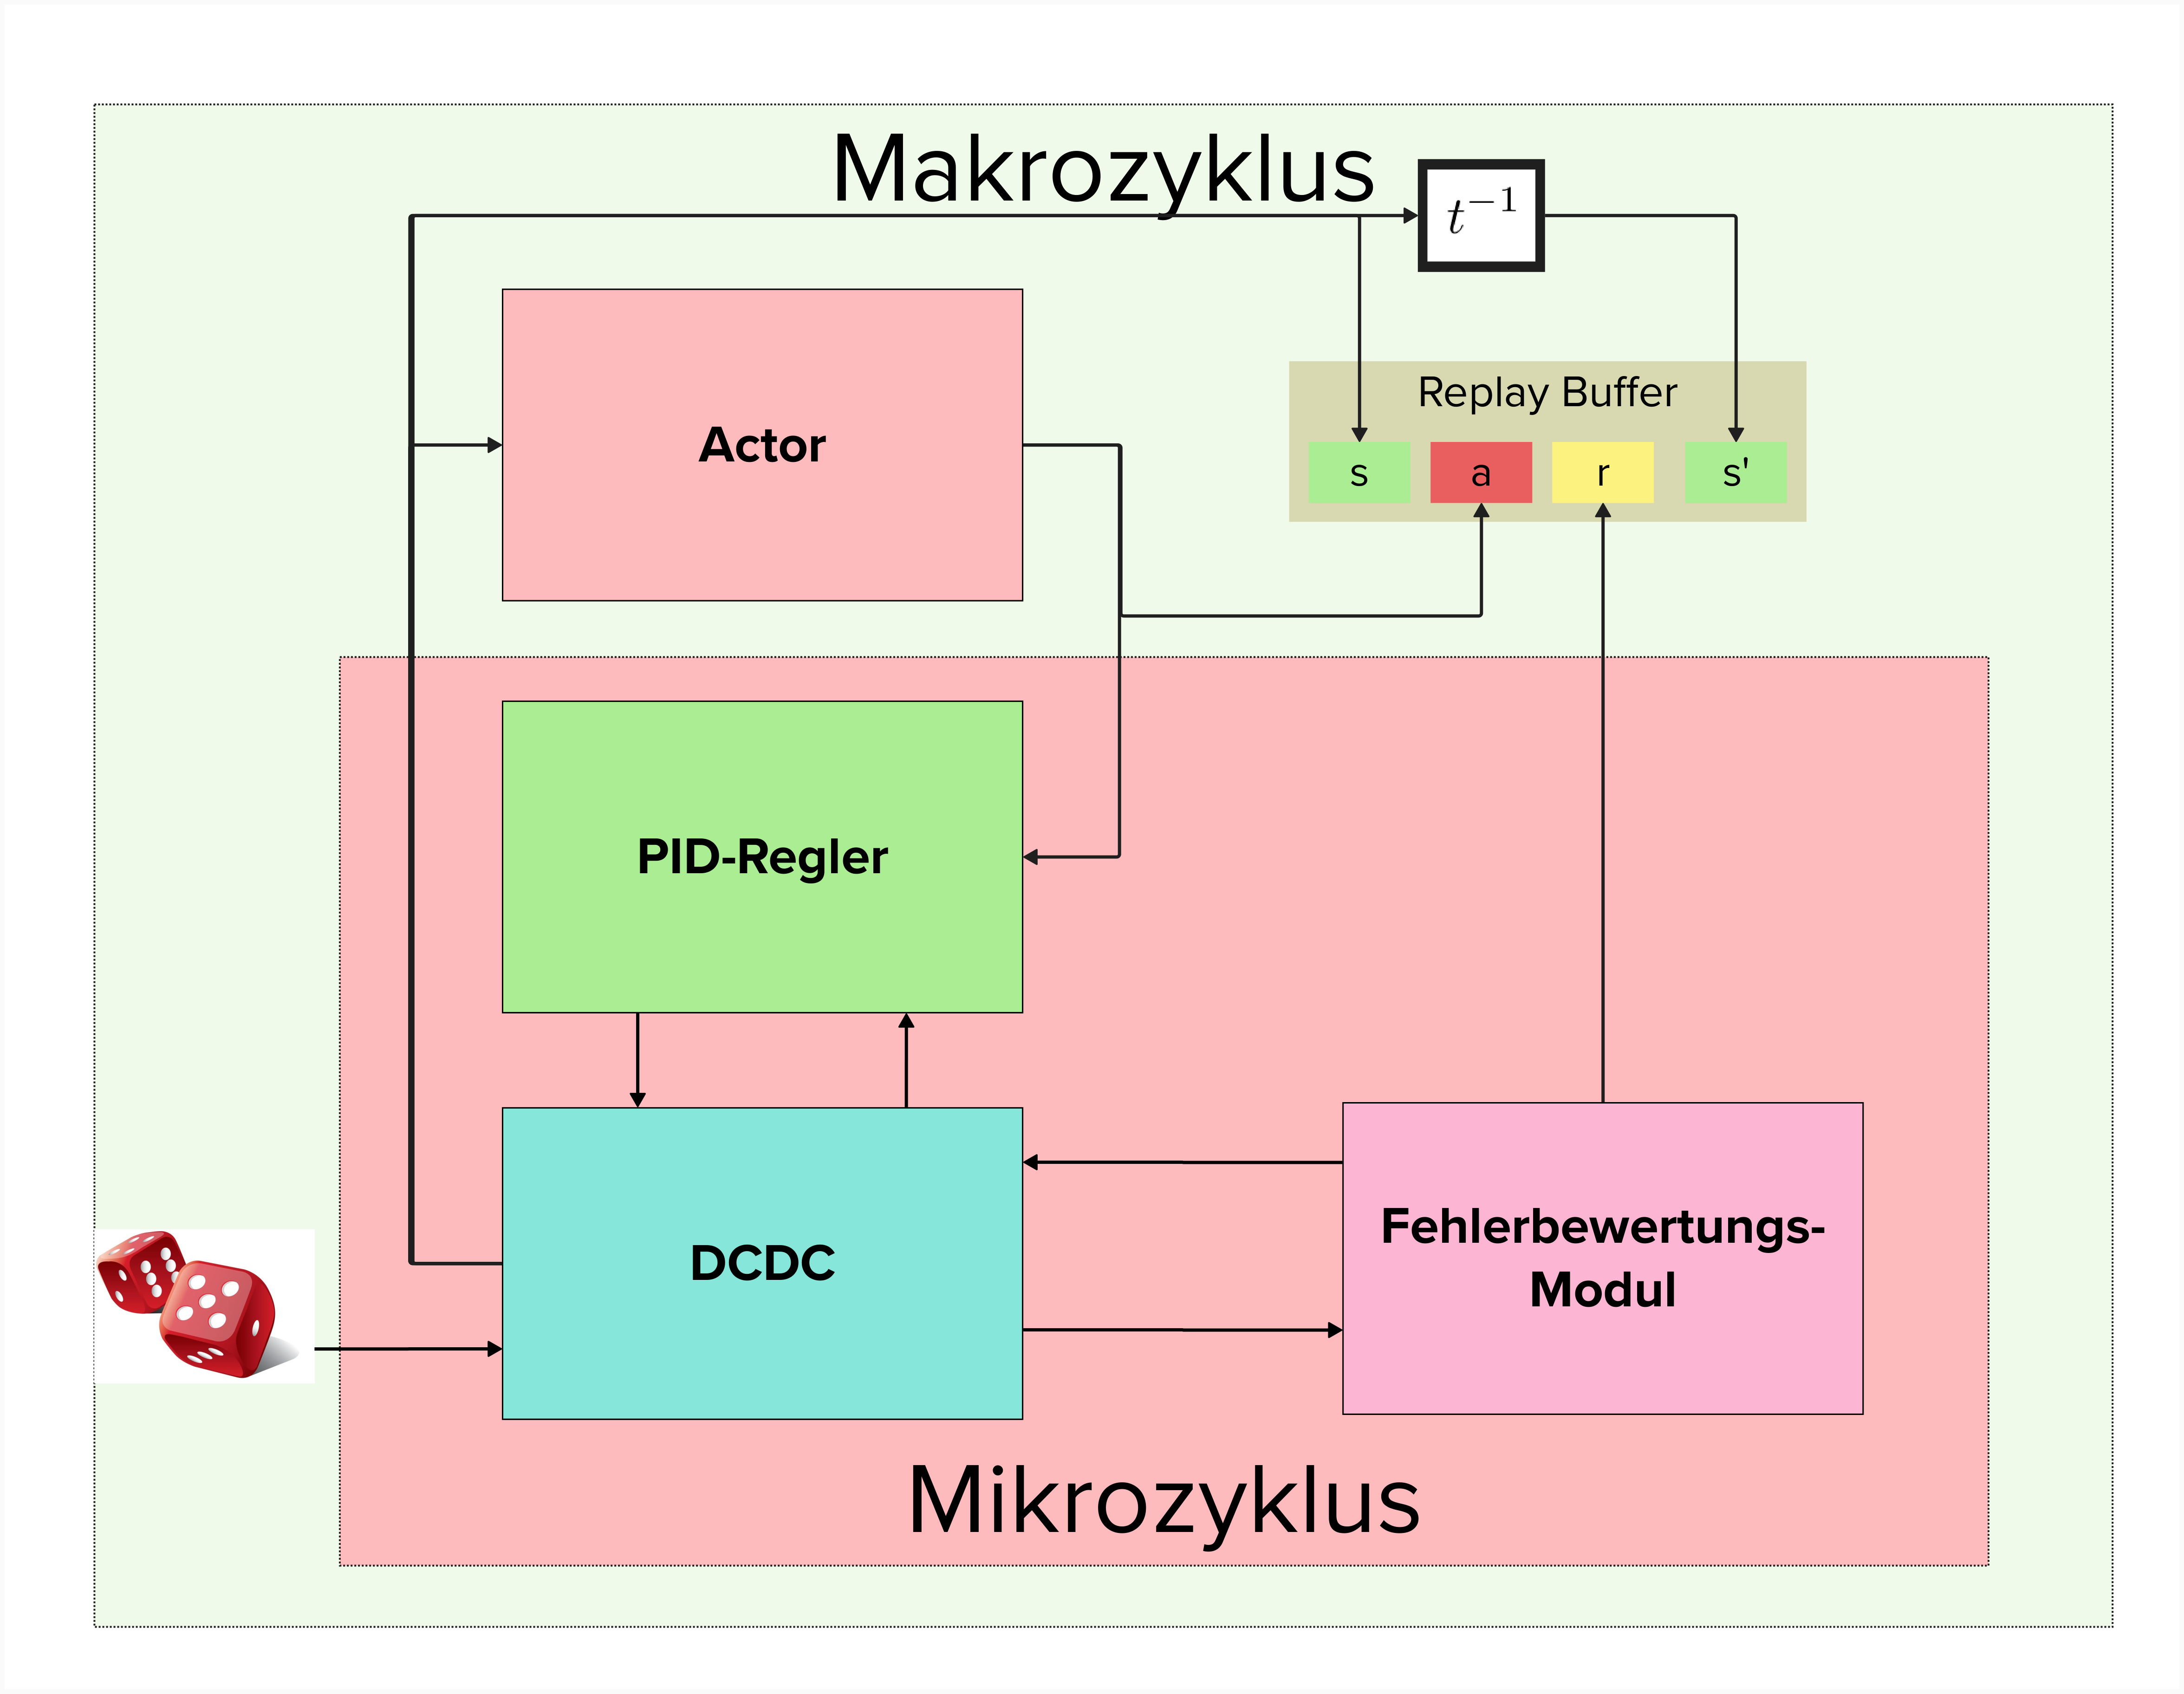
\includegraphics[width=0.8\textwidth]{3Experiment/2Experiment/0Zeitliche_Dimensio.png}
\caption{Visualisierung des Mikro- und Makrozyklus mit Darstellung der zeitlichen Unterteilung in zwei Dimensionen.}
\label{fig:makrozyklus}
\end{figure}

